\documentclass[12pt,a4paper]{report}

% ---------- Paket dasar ----------
\usepackage[utf8]{inputenc}
\usepackage[T1]{fontenc}
\usepackage[indonesian]{babel}
\addto\captionsindonesian{\renewcommand{\bibname}{Referensi}}

% ---------- Paket matematika & gambar ----------
\usepackage{amsmath,amssymb}
\usepackage{graphicx}
\usepackage{caption}
\usepackage{subcaption}
\usepackage{float}
\bibliographystyle{IEEEtran}
\makeatletter
\def\bstctlcite{\@ifnextchar[{\@bstctlcite}{\@bstctlcite[@auxout]}}
\def\@bstctlcite[#1]#2{\@bsphack\@for\@citeb:=#2\do{%
  \edef\@citeb{\expandafter\@firstofone\@citeb}%
  \if@filesw\immediate\write\csname #1\endcsname{\string\citation{\@citeb}}\fi}%
  \@esphack}
\makeatother

% ---------- Paket lain ----------
\usepackage[most]{tcolorbox}
\usepackage{hyperref}
\usepackage{fancyhdr}
\usepackage{titlesec}
\usepackage{longtable}
\usepackage{array}
\usepackage{booktabs}
\usepackage{multirow}
\usepackage[table]{xcolor}
\usepackage{listings}
\usepackage{enumitem}
\usepackage{adjustbox}
\emergencystretch=3em

\setlength{\headheight}{10pt}
\setlength{\headsep}{55pt}
\setlength{\footskip}{28pt}
\usepackage[a4paper,top=3cm,bottom=3cm,left=3cm,right=3cm]{geometry}

% Gambar dari folder public dan dari folder output repository
\graphicspath{{public/}{public/figures/}{../output/}}

% ---------- Listing kode Python ----------
\lstdefinestyle{py}{
	language=Python,
	basicstyle=\ttfamily\scriptsize,
	keywordstyle=\color{blue!70!black}\bfseries,
	commentstyle=\color{gray}\itshape,
	stringstyle=\color{teal!70!black},
	numbers=left,
	numberstyle=\tiny\color{gray},
	frame=single,
	rulecolor=\color{gray!50},
	breaklines=true,
	showstringspaces=false,
	tabsize=4,
	columns=fullflexible,
	keepspaces=true,
	literate={α}{{$\alpha$}}1 {Σ}{{$\Sigma$}}1,
}
% Baris komentar Python tidak ditampilkan: dilewati lewat linerange pada setiap \lstinputlisting.
% Jika kode di src/ berubah, sesuaikan nomor baris pada linerange.
\lstset{style=py}
\renewcommand{\lstlistingname}{Kode}

% ---------- Penanda bagian yang belum selesai ----------
% Hapus semua \todo{...} sebelum laporan dikumpulkan.
\newtcolorbox{todobox}{colback=orange!8,colframe=orange!70!black,boxrule=0.6pt,arc=2pt,left=4pt,right=4pt,top=2pt,bottom=2pt,fontupper=\small}
\newcommand{\todo}[1]{\begin{todobox}\textbf{TODO:} #1\end{todobox}}

% --- Pengaturan header & footer ---
\pagestyle{fancy}
\fancyhf{}

\fancypagestyle{plain}{%
	\fancyhf{}%
	\fancyhead[L]{%
		
\includegraphics[height=1.1cm]{logo-itb}\hspace{0.3cm}%
		
\includegraphics[height=1.1cm]{logo-stei}\hspace{0.3cm}%
	}%
	\fancyhead[R]{%
		\begin{minipage}{9cm}
			\raggedleft\bfseries IF3170 Inteligensi Artifisial\\
			\normalsize Laporan Tugas Besar 2\\
			\itshape Semester I 2026/2027
		\end{minipage}
	}%
	\renewcommand{\headrulewidth}{0.4pt}%
	\fancyfoot[L]{\small v1.0}%
	\fancyfoot[C]{\small Halaman \thepage}%
	\fancyfoot[R]{\small }%
	\renewcommand{\footrulewidth}{0.4pt}%
}

\fancyhead[L]{%
	
\includegraphics[height=1.5cm]{logo-itb}\hspace{0.3cm}%
	
\includegraphics[height=1.5cm]{logo-stei}\hspace{0.3cm}%
}

\fancyhead[R]{%
	\begin{minipage}{9cm}
		\raggedleft\bfseries IF3170 Inteligensi Artifisial\\
		\normalsize Laporan Tugas Besar 2\\
		\itshape Semester I 2026/2027
	\end{minipage}
}

\renewcommand{\headrulewidth}{0.4pt}
\fancyfoot[L]{\small v1.0}
\fancyfoot[C]{\small Halaman \thepage}
\fancyfoot[R]{\small }
\renewcommand{\footrulewidth}{0.4pt}

\begin{document}
\bstctlcite{IEEEexample:BSTcontrol}

	% ================= Cover =================
	\begin{titlepage}
		\thispagestyle{empty}
		\centering

		{\LARGE \textbf{Tugas Besar 2}\par}
		\vspace{0.2cm}
		{\LARGE \textbf{Kelompok G08 - Teazzi}\par}
		\vspace{0.8cm}
		{\large IF3170 Inteligensi Artifisial\par}
		\vspace{0.2cm}
		{\large Klasifikasi Pembatalan Pemesanan Hotel\\dengan Algoritma \textit{Supervised Learning}\par}
		\vspace{0.2cm}
		{\large Semester I Tahun 2026/2027\par}

		\vspace{1.0cm}
		% Taruh foto kelompok di docs/public/foto-kelompok.png; jika tidak ada, logo ITB dipakai.
		\IfFileExists{public/foto-kelompok.png}{%
			\includegraphics[width=0.75\textwidth,height=7cm,keepaspectratio]{foto-kelompok}%
		}{%
			
\includegraphics[height=4.5cm]{logo-itb}%
		}\par

		\vspace{0.8cm}
		{\bfseries Disusun oleh:\par}
		\vspace{0.2cm}
		\textbf{Kelompok G08 - Teazzi}
		\vspace{0.5cm} \\
		\begin{tabular}{l l}
			Jason Edward Salim & (13524034) \\
			Stefani Angeline Oroh & (13524064) \\
			Bryan Pratama Putra Hendra & (13524067) \\
			Angelina Andra Alanna & (13524079) \\
			Michael James Liman & (13524106) \\
		\end{tabular}

		\vfill
		Laboratorium Artificial Intelligence\par
		Program Studi Teknik Informatika\par
		Sekolah Teknik Elektro dan Informatika\par
		Institut Teknologi Bandung\par

	\end{titlepage}

	\clearpage
	\pagestyle{fancy}

	\tableofcontents
	\clearpage
	\listoftables
	\clearpage
	\listoffigures
	\clearpage

	\chapter{Deskripsi Persoalan}
	\section{Latar Belakang}

Pemesanan hotel yang dibatalkan, terutama menjelang tanggal kedatangan,
meninggalkan kamar kosong yang sulit dijual kembali. Jika pembatalan dapat
diperkirakan sejak awal, hotel dapat mengambil langkah pencegahan, misalnya
meminta deposit atau menghubungi tamu lebih awal. Tugas ini membangun model
klasifikasi biner untuk memprediksi apakah sebuah pemesanan akan dibatalkan
(\texttt{is\_canceled} $=1$) atau tidak (\texttt{is\_canceled} $=0$) berdasarkan
data pemesanan~\cite{asisten2026spek}.

Kedua jenis kesalahan prediksi berdampak berbeda bagi hotel. \textit{False
negative} terjadi ketika pemesanan yang akhirnya dibatalkan diprediksi tidak
batal. Hotel tidak mengambil langkah apa pun, dan kamar tersebut berisiko kosong
setelah pembatalan terjadi. \textit{False positive} terjadi ketika pemesanan yang
sebenarnya datang diprediksi batal. Jika hotel menanggapinya dengan menjual kamar
yang sama ke tamu lain (\textit{overbooking}), tamu yang datang bisa tidak
mendapat kamar. Jika hotel menanggapinya dengan meminta deposit atau menghubungi
tamu, tamu yang sebenarnya akan datang ikut terbebani.

\textit{Dataset} ini tidak memuat biaya kedua jenis kesalahan tersebut sehingga
laporan ini tidak memberi bobot yang berbeda pada keduanya. Model dievaluasi
dengan \textit{macro F1-score} (Subbab~\ref{sec:distribusi-kelas}), yang
memperhitungkan kesalahan pada kedua kelas secara seimbang. Jika hotel mengetahui
kerugian masing-masing kesalahan, ambang keputusan model dapat digeser untuk
mengurangi jenis kesalahan yang lebih mahal.

\section{\textit{Dataset}}

\textit{Dataset} terdiri atas \texttt{data/train.csv} yang berlabel dan
\texttt{data/test.csv} yang tidak berlabel. Prediksi untuk data uji disimpan
dengan format \texttt{data/sample\_submission.csv}, yaitu kolom \texttt{id} dan
\texttt{is\_canceled}.

\begin{table}[H]
	\centering
	\caption{Ukuran \textit{dataset}}
	\label{tab:ukuran}
	\begin{tabular}{l r r}
		\toprule
		\textbf{Berkas} & \textbf{Baris} & \textbf{Kolom} \\
		\midrule
		\texttt{train.csv} & 27.373 & 19 (17 fitur, \texttt{id}, \texttt{is\_canceled}) \\
		\texttt{test.csv}  & 6.844  & 18 (17 fitur, \texttt{id}) \\
		\bottomrule
	\end{tabular}
\end{table}

\begin{table}[H]
	\centering
	\caption{Atribut \textit{dataset}}
	\label{tab:atribut}
	\small
	\begin{tabular}{l l p{6cm}}
		\toprule
		\textbf{Atribut} & \textbf{Tipe} & \textbf{Keterangan} \\
		\midrule
		\texttt{num\_adults}, \texttt{num\_children} & numerik & Jumlah tamu dewasa dan anak \\
		\texttt{weekend\_nights}, \texttt{weekday\_nights} & numerik & Jumlah malam akhir pekan dan hari kerja \\
		\texttt{meal\_package} & kategorikal & Room Only, Breakfast, Half Board, Full Board \\
		\texttt{needs\_parking} & biner & Tamu membutuhkan tempat parkir \\
		\texttt{room\_category} & kategorikal & Type A-G \\
		\texttt{days\_before\_arrival} & numerik & Selisih hari antara pemesanan dan kedatangan (\textit{lead time}) \\
		\texttt{arrival\_year/month/day} & numerik & Tanggal kedatangan (2023-2024) \\
		\texttt{booking\_channel} & kategorikal & Online Travel Agent, Offline Agent, Corporate, Complimentary, Airline \\
		\texttt{is\_returning\_guest} & biner & Tamu pernah menginap sebelumnya \\
		\texttt{prior\_cancellations} & numerik & Jumlah pembatalan sebelumnya \\
		\texttt{prior\_completed\_bookings} & numerik & Jumlah pemesanan sebelumnya yang tidak dibatalkan \\
		\texttt{nightly\_rate\_idr} & numerik & Harga kamar per malam (rupiah) \\
		\texttt{special\_requests} & numerik & Jumlah permintaan khusus \\
		\midrule
		\texttt{is\_canceled} & biner & Target: 1 jika pemesanan dibatalkan \\
		\bottomrule
	\end{tabular}
\end{table}

\section{Pemahaman Data}

Analisis eksploratif dibuat dengan fungsi di \texttt{src/eda.py} dan dijalankan
pada bagian \textit{Data Understanding} di \texttt{src/main.ipynb}.

\subsection{Distribusi Kelas}
\label{sec:distribusi-kelas}

Dari 27.373 baris data latih, 18.404 baris (67,2\%) tidak batal dan 8.969 baris
(32,8\%) batal (Gambar~\ref{fig:target}). Perbandingan kedua kelas sekitar 2:1.
Karena itu, model dievaluasi dengan \textit{macro F1-score} agar kinerja pada kelas
batal yang lebih sedikit berbobot sama dengan kelas tidak batal. \textit{Macro
F1-score} adalah rata-rata F1 kedua kelas.

\begin{figure}[H]
	\centering
	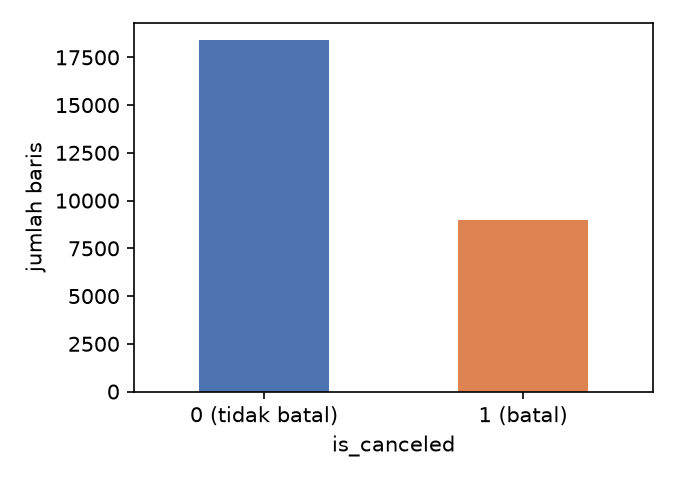
\includegraphics[width=0.55\textwidth]{target_distribution}
	\caption{Distribusi kelas \texttt{is\_canceled} pada data latih}
	\label{fig:target}
\end{figure}

\subsection{Nilai Hilang dan Duplikat}

Delapan atribut memiliki nilai hilang dengan proporsi yang hampir sama pada data
latih dan data uji (Tabel~\ref{tab:missing}). Imputasi yang di-\textit{fit} pada
data latih pun dapat diterapkan langsung ke data uji. Data latih memuat 66 baris
duplikat (seluruh fitur identik), data uji memuat 3 baris, dan gabungan keduanya
memuat 109 baris.

\begin{table}[H]
	\centering
	\caption{Persentase nilai hilang per atribut}
	\label{tab:missing}
	\begin{tabular}{l r r}
		\toprule
		\textbf{Atribut} & \textbf{Latih (\%)} & \textbf{Uji (\%)} \\
		\midrule
		\texttt{num\_children}        & 11,09 & 10,91 \\
		\texttt{special\_requests}    & 9,13  & 8,66 \\
		\texttt{nightly\_rate\_idr}   & 7,45  & 7,89 \\
		\texttt{meal\_package}        & 6,43  & 6,46 \\
		\texttt{days\_before\_arrival}& 4,10  & 4,24 \\
		\texttt{needs\_parking}       & 3,95  & 3,61 \\
		\texttt{room\_category}       & 3,66  & 3,54 \\
		\texttt{num\_adults}          & 2,96  & 2,63 \\
		\bottomrule
	\end{tabular}
\end{table}

\subsection{Sebaran Fitur dan Pencilan}

Sebagian besar fitur numerik menceng ke kanan. Median
\texttt{days\_before\_arrival} adalah 58 hari dengan maksimum 448 hari. Median
\texttt{nightly\_rate\_idr} adalah Rp1.644.000 dengan maksimum Rp9.165.000, dan
beberapa baris memiliki harga Rp0. Hampir semua nilai
\texttt{prior\_cancellations} dan \texttt{prior\_completed\_bookings} adalah 0.
Distribusi kategori juga timpang: Type B mencakup 75\% nilai
\texttt{room\_category}, Full Board hanya muncul empat kali pada
\texttt{meal\_package}, dan Airline hanya muncul 88 kali pada
\texttt{booking\_channel}.

\subsection{Korelasi dengan Target}

Gambar~\ref{fig:korelasi} menunjukkan korelasi Pearson antara setiap fitur numerik
dan target. Korelasi positif terbesar dimiliki \texttt{days\_before\_arrival}
(0,44): pemesanan yang dibuat jauh hari lebih sering dibatalkan. Korelasi negatif
terbesar dimiliki \texttt{special\_requests} ($-0{,}26$): tamu yang mengajukan
permintaan khusus lebih jarang membatalkan pemesanan. \texttt{arrival\_year} (0,18)
dan \texttt{nightly\_rate\_idr} (0,13) juga berkorelasi positif dengan pembatalan.

\begin{figure}[H]
	\centering
	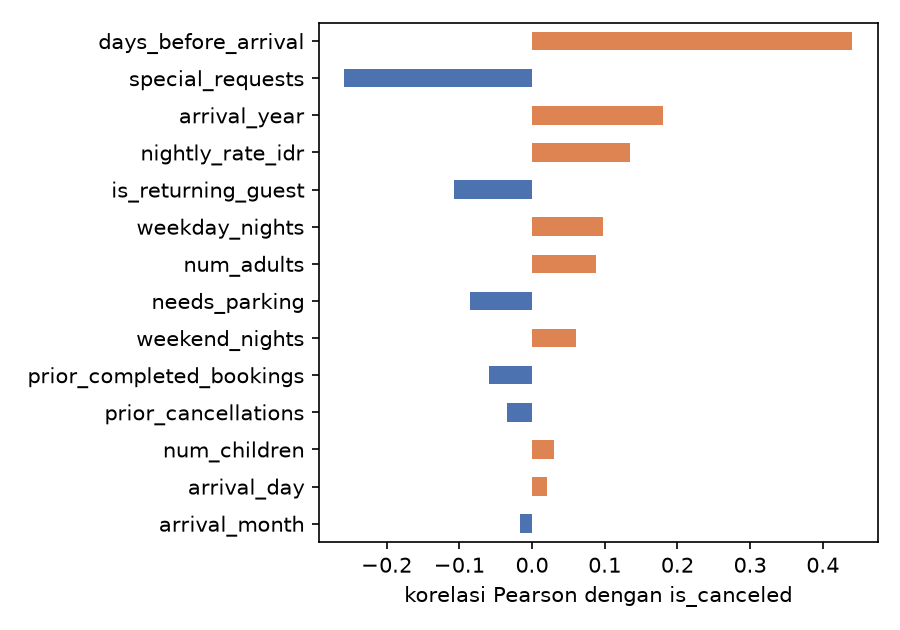
\includegraphics[width=0.75\textwidth]{correlation}
	\caption{Korelasi fitur numerik dengan \texttt{is\_canceled}}
	\label{fig:korelasi}
\end{figure}

\subsection{Rasio Pembatalan per Kategori}

Gambar~\ref{fig:target-rate} menunjukkan rasio pembatalan untuk setiap nilai
\texttt{booking\_channel}, \texttt{meal\_package}, \texttt{room\_category}, dan
\texttt{arrival\_month}. Gambar ini dibuat dengan fungsi \texttt{target\_rate} di
\texttt{src/eda.py}. Garis putus-putus menandai rasio pembatalan seluruh data
latih (32,8\%).

\begin{figure}[H]
	\centering
	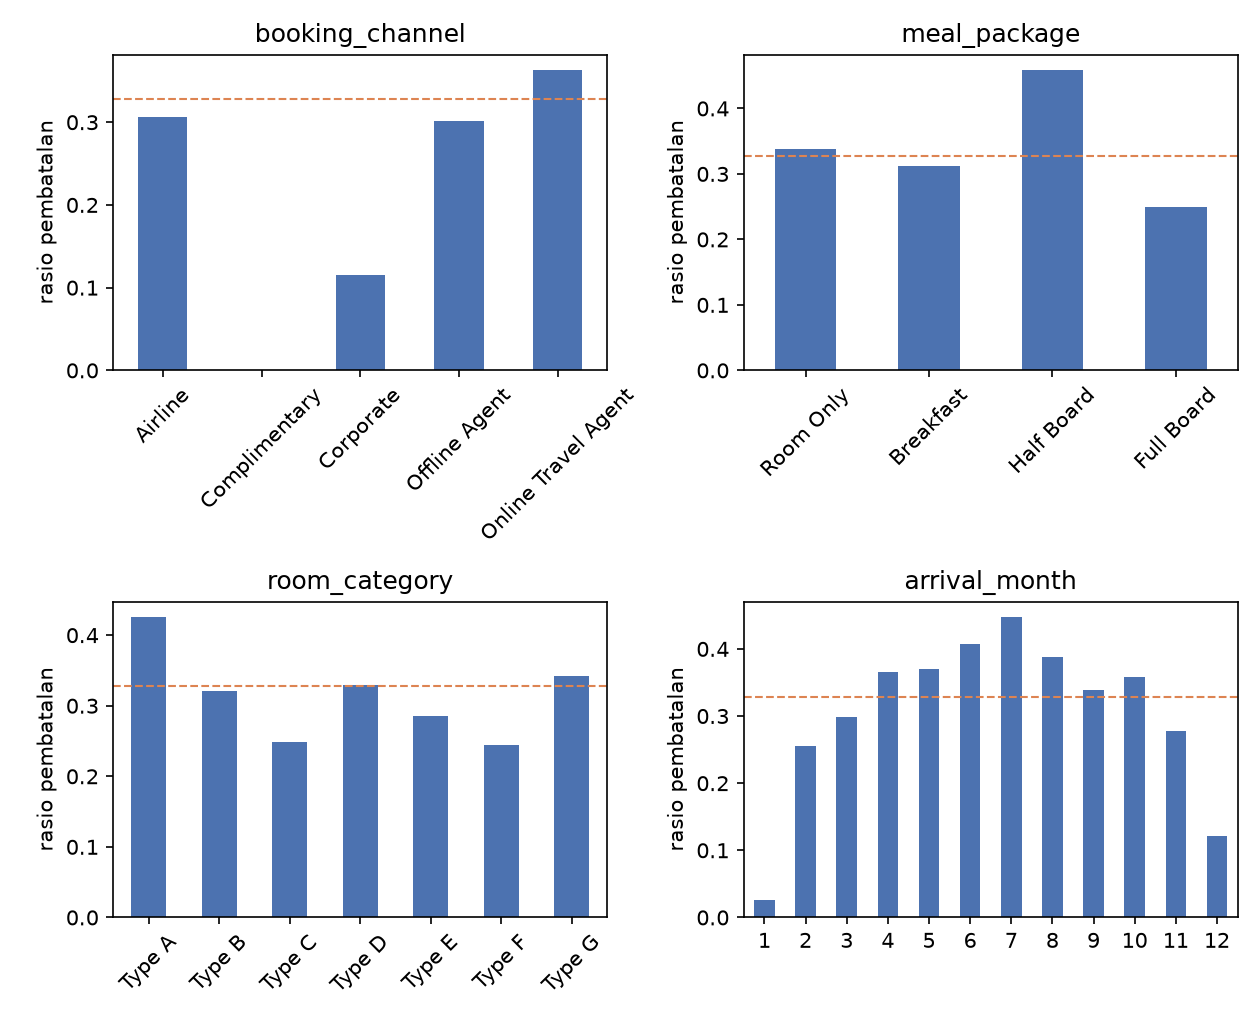
\includegraphics[width=0.95\textwidth]{target_rate}
	\caption{Rasio pembatalan per kategori pada data latih}
	\label{fig:target-rate}
\end{figure}

Perbedaan terbesar terlihat pada \texttt{booking\_channel}. Online Travel Agent,
kanal dengan 17.511 pemesanan, memiliki rasio pembatalan 36,4\%, sedangkan
Offline Agent memiliki rasio 30,2\%. Rasio pada Corporate hanya 11,5\%, dan tidak
satu pun dari 301 pemesanan Complimentary dibatalkan. Airline memiliki rasio
30,7\%, tetapi hanya berisi 88 pemesanan.

Pada \texttt{meal\_package}, Half Board memiliki rasio pembatalan tertinggi
(45,9\% dari 2.242 pemesanan). Room Only (33,8\%) dan Breakfast (31,1\%) dekat
dengan rasio keseluruhan. Rasio Full Board (25,0\%) tidak dapat ditafsirkan karena
hanya berasal dari empat pemesanan.

Pada \texttt{room\_category}, Type A memiliki rasio tertinggi (42,6\% dari 699
pemesanan), sedangkan Type C (24,9\%) dan Type F (24,4\%) memiliki rasio
terendah. Type B dan Type G, yang bersama-sama mencakup 91\% data, memiliki rasio
32,1\% dan 34,2\%. Selisih antartipe kamar lebih kecil daripada selisih antarkanal
pemesanan.

Rasio pembatalan per \texttt{arrival\_month} membentuk pola musiman. Rasio naik
dari 2,6\% pada Januari ke puncaknya, 44,8\%, pada Juli, lalu turun ke 12,1\% pada
Desember. Desember dan Januari sama-sama memiliki rasio rendah meskipun nomor
bulannya berjauhan. Hal tersebut sejalan dengan \textit{encoding} siklik
(\texttt{month\_sin} dan \texttt{month\_cos}) pada Bab~3 yang menempatkan kedua
bulan itu berdekatan. Plot ini tidak
menunjukkan penyebab pola tersebut. Bulan kedatangan dapat berkaitan dengan fitur
lain, misalnya \textit{lead time} atau tahun kedatangan.


	\chapter{Pembahasan: Implementasi Algoritma}
	Program ditulis dalam Python dan disimpan di folder \texttt{src/}. Model
\textit{from scratch} hanya memakai NumPy~\cite{numpy2026docs}. Scikit-learn dipakai untuk pembagian
data, perhitungan metrik, dan model pembanding~\cite{sklearn2026docs}. Alur
kerja mengikuti tahapan CRISP-DM dan dijalankan dari \texttt{src/main.ipynb}.
Potongan kode pada bab ini diambil langsung dari \textit{repository}.

\section{Struktur Program}

\begin{table}[H]
	\centering
	\caption{Modul program}
	\label{tab:modul}
	\begin{tabular}{l p{7.6cm}}
		\toprule
		\textbf{Modul} & \textbf{Isi} \\
		\midrule
		\texttt{config.py} & Konstanta global (\textit{seed}, \textit{path}, nama kolom, rasio pembagian data, jumlah \textit{fold}) \\
		\texttt{eda.py} & Fungsi analisis eksploratif: tipe data, nilai hilang, duplikat, histogram, \textit{boxplot}, pencilan IQR, korelasi \\
		\texttt{preprocessing.py} & Pembagian data, \texttt{Preprocessor}, rekayasa fitur, PCA, dan \texttt{Pipeline} (seleksi fitur, PCA, model) \\
		\texttt{validation.py} & \textit{Hold-out}, \textit{k-fold}, \textit{tuning}, \textit{confusion matrix}, analisis kesalahan, \textit{resampling}, dan pembuatan berkas prediksi \\
		\texttt{models/base.py} & Antarmuka \texttt{BaseModel}: \texttt{fit}, \texttt{predict}, \texttt{set\_params}, \texttt{save}, \texttt{load} \\
		\texttt{models/knn.py} & K-Nearest Neighbors \\
		\texttt{models/logistic\_regression.py} & Logistic Regression \\
		\texttt{models/svm.py} & Support Vector Machine (SMO) \\
		\texttt{models/dtl.py} & Decision Tree Learning \\
		\texttt{models/bayes\_network.py} & Bayesian Network \\
		\texttt{main.ipynb} & \textit{Notebook} utama yang menjalankan seluruh tahapan CRISP-DM \\
		\bottomrule
	\end{tabular}
\end{table}

\section{Antarmuka Model}

Semua model \textit{from scratch} merupakan turunan \texttt{BaseModel}.
\texttt{fit(X, y)} menerima \textit{array} NumPy dan mengembalikan \texttt{self},
sedangkan \texttt{predict(X)} mengembalikan label 0 atau 1. Antarmuka ini sama
dengan antarmuka scikit-learn. Akibatnya, fungsi validasi, \textit{tuning}, dan
\texttt{Pipeline} dapat dipakai, baik untuk model \textit{from scratch} maupun
model pembanding, tanpa perubahan. Model yang sudah dilatih disimpan dan dimuat
kembali dengan \texttt{pickle}.

\lstinputlisting[caption={Antarmuka model (\texttt{src/models/base.py})},linerange={1-3,5-24}]{../src/models/base.py}

\section{K-Nearest Neighbors}
\label{sec:knn}

\todo{Implementasi \texttt{KNN.fit} dan \texttt{KNN.predict} di
\texttt{src/models/knn.py} belum selesai. Parameter yang sudah disiapkan:
\texttt{k}, \texttt{metric} (\texttt{euclidean}, \texttt{manhattan},
\texttt{minkowski}), dan \texttt{p}. Jelaskan cara kerja, fungsi/kelas, dan
sertakan potongan kode setelah implementasi selesai.}

\section{Logistic Regression}
\label{sec:lr}

\todo{Implementasi \texttt{LogisticRegression.fit} dan \texttt{predict} di
\texttt{src/models/logistic\_regression.py} belum selesai. Parameter yang sudah
disiapkan: \texttt{lr}, \texttt{n\_iter}, \texttt{reg} (L1/L2), dan \texttt{lam}.
Jelaskan fungsi sigmoid, \textit{log-loss}, \textit{gradient descent}, dan
regularisasi beserta potongan kode.}

\section{Support Vector Machine}
\label{sec:svm}

\subsection{Formulasi}

SVM dengan \textit{soft margin} mencari \textit{hyperplane} pemisah dengan margin
terbesar dan mengizinkan sebagian sampel melanggar margin.
Implementasi ini menyelesaikan bentuk dualnya. Untuk label $y_i\in\{-1,+1\}$ dan
fungsi kernel $K$, masalah dualnya adalah
\begin{equation}
	\max_{\alpha}\ \sum_{i}\alpha_i-\frac{1}{2}\sum_{i}\sum_{j}\alpha_i\alpha_j y_i y_j K(x_i,x_j)
	\quad\text{dengan}\quad 0\le\alpha_i\le C,\ \ \sum_i\alpha_i y_i=0 .
\end{equation}
Parameter $C$ menentukan besarnya hukuman untuk pelanggaran margin. Setelah
$\alpha$ diperoleh, prediksi dihitung dari \textit{support vector}, yaitu sampel
dengan $\alpha_i>0$:
\begin{equation}
	f(x)=\sum_{i\in SV}\alpha_i y_i K(x_i,x)+b,\qquad \hat{y}=\begin{cases}1 & f(x)\ge 0\\ 0 & f(x)<0\end{cases}
\end{equation}
Implementasi mendukung empat kernel (Tabel~\ref{tab:kernel}). Nama \texttt{rbf}
dan \texttt{gaussian} merujuk ke kernel yang sama.

\begin{table}[H]
	\centering
	\caption{Kernel SVM yang didukung}
	\label{tab:kernel}
	\begin{tabular}{l l}
		\toprule
		\textbf{Kernel} & $K(a,b)$ \\
		\midrule
		\texttt{linear} & $a^\top b$ \\
		\texttt{poly} & $(\gamma\, a^\top b + c_0)^{d}$ \\
		\texttt{rbf} / \texttt{gaussian} & $\exp(-\gamma\lVert a-b\rVert^2)$ \\
		\texttt{sigmoid} & $\tanh(\gamma\, a^\top b + c_0)$ \\
		\bottomrule
	\end{tabular}
\end{table}

\lstinputlisting[caption={Parameter dan fungsi kernel (\texttt{src/models/svm.py})},linerange={5-5,7-10,12-23,25-28}]{../src/models/svm.py}

\subsection{Sequential Minimal Optimization}

Masalah dual diselesaikan dengan \textit{Sequential Minimal Optimization}
(SMO). Setiap iterasi SMO hanya mengubah dua variabel, yaitu
$\alpha_i$ dan $\alpha_j$. Subproblem dua variabel ini dapat diselesaikan secara
analitik tanpa melanggar $\sum_i\alpha_i y_i=0$. Pasangan $(i,j)$ dipilih dengan
\textit{second-order working set selection} melalui langkah
berikut.
\begin{enumerate}
	\item Untuk setiap sampel, simpan $u_k=\sum_l\alpha_l y_l K(x_l,x_k)$ dan
	$g_k=y_k-u_k$. Himpunan $I_{\text{up}}$ berisi sampel yang $\alpha$-nya masih
	dapat bergerak searah $y_k$ positif. Himpunan $I_{\text{low}}$ berisi sampel
	yang $\alpha$-nya dapat bergerak ke arah sebaliknya.
	\item Pilih $i=\arg\max_{k\in I_{\text{up}}} g_k$, yaitu sampel yang paling
	melanggar kondisi KKT.
	\item Hentikan pelatihan jika $g_i-\min_{k\in I_{\text{low}}}g_k<\texttt{tol}$
	karena kondisi KKT sudah terpenuhi.
	\item Di antara sampel $I_{\text{low}}$ dengan $g_j<g_i$, pilih $j$ yang
	memaksimalkan kenaikan objektif $(g_i-g_j)^2/(K_{ii}+K_{jj}-2K_{ij})$.
	\item Perbarui $\alpha_j$ dengan langkah Newton
	$\alpha_j+y_j(g_j-g_i)/\eta$, dengan $\eta=K_{ii}+K_{jj}-2K_{ij}$, lalu potong
	hasilnya ke batas $[L,H]$ agar $0\le\alpha\le C$. Sesuaikan $\alpha_i$ agar
	$\sum\alpha y$ tidak berubah.
	\item Perbarui $u$ secara inkremental dengan baris kernel ke-$i$ dan ke-$j$.
\end{enumerate}
Setiap iterasi hanya menghitung dua baris kernel, sedangkan matriks kernel penuh
berukuran $n\times n$ tidak pernah disimpan. Untuk 21.857 baris data latih, matriks
penuh dalam \textit{float64} membutuhkan sekitar 3,8 GB memori. Untuk kernel
Gaussian, norma kuadrat setiap baris (\texttt{sq}) dihitung sekali di awal
sehingga satu baris kernel cukup dihitung dengan satu perkalian matriks-vektor.
Fungsi \texttt{snap} membulatkan nilai $\alpha$ yang sangat dekat dengan 0 atau
$C$ agar status \textit{bound} tidak berganti-ganti akibat galat
\textit{floating point}.

Setelah konvergen, bias $b$ dihitung sebagai rata-rata $g_k$ pada \textit{free
support vector} ($0<\alpha_k<C$) karena sampel tersebut terletak tepat di margin.
Untuk kernel linear, bobot $w=\sum_i\alpha_i y_i x_i$ disimpan di
\texttt{coef\_}. Prediksi kernel linear cukup dihitung sebagai $Xw+b$, dan nilai
$|w|$ dipakai untuk seleksi fitur (Subbab~\ref{sec:seleksi}).

\lstinputlisting[caption={Pelatihan SVM dengan SMO (\texttt{src/models/svm.py})},linerange={30-72}]{../src/models/svm.py}

\lstinputlisting[caption={Fungsi keputusan dan prediksi SVM (\texttt{src/models/svm.py})},linerange={75-83}]{../src/models/svm.py}

\section{Decision Tree Learning}
\label{sec:dtl}

\todo{Implementasi \texttt{DTL.fit} dan \texttt{DTL.predict} di
\texttt{src/models/dtl.py} belum selesai. Parameter yang sudah disiapkan:
\texttt{criterion} (\texttt{entropy}/\texttt{gini}), \texttt{max\_depth}, dan
\texttt{min\_samples\_split}. Jelaskan perhitungan \textit{information gain},
penanganan atribut kontinu, kriteria berhenti, dan potongan kode. Jika DTL
menyediakan \texttt{feature\_importances\_}, \texttt{Pipeline} otomatis dapat
memakainya untuk seleksi fitur.}

\section{Bayesian Network}
\label{sec:bn}

\todo{Implementasi \texttt{BayesNetwork.fit} dan \texttt{predict} di
\texttt{src/models/bayes\_network.py} belum selesai. Parameter yang sudah
disiapkan: \texttt{n\_bins} untuk diskretisasi fitur kontinu. Jelaskan cara
membangun struktur jaringan, estimasi \textit{conditional probability table}
(beserta \textit{smoothing}), dan inferensi posterior.}

\section{Validasi dan Utilitas Eksperimen}

Seluruh evaluasi dijalankan melalui fungsi di \texttt{src/validation.py} agar
semua model diuji dengan prosedur yang sama. Fungsi yang tersedia adalah sebagai
berikut.
\begin{itemize}
	\item \texttt{holdout} melatih model pada \texttt{X\_train} dan mengevaluasinya
	pada \texttt{X\_val}.
	\item \texttt{kfold} menjalankan \textit{stratified 5-fold cross validation}
	pada \texttt{X\_train} serta melaporkan rata-rata dan simpangan baku
	\textit{macro F1}.
	\item \texttt{tune} menjalankan \textit{grid search} dengan skor
	\textit{k-fold}, lalu \texttt{best} mengambil parameter terbaik.
	\item \texttt{resample} menerapkan SMOTE atau
	\textit{random undersampling} hanya pada data latih di setiap \textit{fold}.
	Data validasi tidak pernah berisi sampel sintetis.
	\item \texttt{confusion}, \texttt{report}, \texttt{misclassified}, dan
	\texttt{importance} dipakai untuk analisis kesalahan.
	\item \texttt{submit} melatih ulang model pada seluruh data berlabel, menulis
	prediksi ke \texttt{output/<model>\_<timestamp>.csv}, dan menyimpan model ke
	berkas \texttt{.pkl}.
\end{itemize}
Setiap model di-\texttt{deepcopy} sebelum dilatih sehingga objek model di
\textit{notebook} tidak berubah setelah validasi. Model yang belum
diimplementasikan (\texttt{NotImplementedError}) dilewati secara otomatis.

\lstinputlisting[caption={\textit{Hold-out} dan \textit{k-fold} (\texttt{src/validation.py})},linerange={13-58}]{../src/validation.py}


	\chapter{Pembahasan: \textit{Data Cleaning} dan \textit{Preprocessing}}
	Seluruh tahap \textit{cleaning} dan \textit{preprocessing} berada di
\texttt{src/preprocessing.py}. Untuk mencegah \textit{data leakage}, data dibagi
terlebih dahulu. Setelah itu, setiap statistik (nilai imputasi, batas pencilan,
daftar kategori, rata-rata, dan simpangan baku) dihitung hanya dari
\texttt{X\_train}, lalu diterapkan apa adanya ke \texttt{X\_val} dan
\texttt{X\_test}.

\section{Pembagian Data}

Fungsi \texttt{split} membagi data latih menjadi 80\% \texttt{X\_train} dan 20\%
\texttt{X\_val} secara \textit{stratified} dengan \textit{seed} 42 sehingga
proporsi kelas batal pada kedua bagian sama. \texttt{X\_val} dipakai untuk
evaluasi \textit{hold-out}, sedangkan \textit{k-fold} dijalankan di dalam
\texttt{X\_train}.

\section{\textit{Data Cleaning}}

\subsection{Duplikat}

Baris dengan seluruh fitur identik dihapus dari \texttt{X\_train} melalui
\texttt{drop\_duplicates}. Duplikat membuat sampel tertentu berbobot ganda. Jika
satu salinan masuk ke \textit{fold} latih dan salinan lain masuk ke \textit{fold}
validasi, skor validasi juga menjadi terlalu tinggi. Duplikat pada \texttt{X\_val}
dan \texttt{X\_test} tidak dihapus karena setiap baris pada kedua data itu tetap
harus diprediksi.

\subsection{Nilai Hilang}

Imputasi dilakukan dalam dua tahap. Pada tahap pertama, \texttt{nightly\_rate\_idr}
diisi dengan median harga per pasangan (\texttt{room\_category},
\texttt{arrival\_month}), dan \texttt{days\_before\_arrival} diisi dengan median
per pasangan (\texttt{booking\_channel}, \texttt{arrival\_month}). Harga kamar
bergantung pada tipe kamar dan musim, sedangkan \textit{lead time} bergantung pada
kanal pemesanan. Karena itu, median kelompok diharapkan lebih mendekati nilai
sebenarnya daripada median global. Kedua fitur ini juga merupakan fitur dengan korelasi
terbesar terhadap target.

Pada tahap kedua, nilai yang masih hilang diisi dengan median untuk fitur numerik
dan modus untuk fitur kategorikal. Median dipilih karena tidak terpengaruh
pencilan dan distribusi fitur yang menceng.

Parameter \texttt{zero\_as\_missing} disediakan untuk memperlakukan nilai 0 sebagai
nilai hilang, misalnya harga kamar Rp0. Data latih memuat 413 baris (1,5\%)
dengan \texttt{nightly\_rate\_idr} bernilai Rp0, dan data uji memuat 85 baris.
Harga terendah berikutnya adalah Rp16.000 sehingga Rp0 terpisah jelas dari harga
lainnya. Sebanyak 267 baris Rp0 berasal dari kanal Complimentary, sedangkan 146
baris lainnya berasal dari Online Travel Agent. Dari 301 pemesanan Complimentary,
267 pemesanan berharga Rp0. Rasio pembatalan baris Rp0 hanya 0,7\%, jauh di bawah
rasio pembatalan baris lain (33,4\%).

Pola ini menunjukkan bahwa Rp0 kemungkinan besar menandai kamar gratis, bukan
harga yang tidak tercatat. Jika Rp0 diganti dengan median, informasi tersebut
hilang. SVM RBF ($C=3$, $\gamma=0{,}1$) dengan kedua pilihan menghasilkan skor
yang setara: \textit{macro F1} \textit{hold-out} 0,8384 dan rata-rata 5-\textit{fold}
0,8328 jika Rp0 dipertahankan, serta 0,8376 dan 0,8329 jika Rp0 dianggap nilai
hilang. Selisih keduanya jauh lebih kecil daripada simpangan baku antar-\textit{fold}
(0,006). Karena skornya setara dan Rp0 memiliki makna yang jelas, konfigurasi
akhir mempertahankan Rp0 sebagai nilai asli (\texttt{zero\_as\_missing} kosong).

\subsection{Pencilan}

Nilai \texttt{days\_before\_arrival} dan \texttt{nightly\_rate\_idr} dibatasi
(\textit{capping}) ke rentang IQR
$[Q_1-1{,}5\,\text{IQR},\ Q_3+1{,}5\,\text{IQR}]$ yang dihitung dari
\texttt{X\_train}. Baris dengan nilai ekstrem tidak dibuang karena baris tersebut
tetap valid dan harus diprediksi. Pembatasan ini mencegah nilai ekstrem
mendominasi jarak pada KNN dan SVM RBF serta \textit{gradient} pada Logistic
Regression.

\section{Rekayasa Fitur}

Fungsi \texttt{engineer} membuat fitur baru hanya dari nilai pada baris yang sama.
Karena tidak memakai statistik dari baris lain, fungsi ini aman diterapkan ke data
mana pun.

\begin{table}[H]
	\centering
	\caption{Fitur hasil rekayasa}
	\label{tab:fitur-baru}
	\small
	\begin{tabular}{l p{8.3cm}}
		\toprule
		\textbf{Fitur} & \textbf{Definisi dan alasan} \\
		\midrule
		\texttt{total\_nights} & \texttt{weekend\_nights} + \texttt{weekday\_nights}; lama menginap total \\
		\texttt{total\_guests} & \texttt{num\_adults} + \texttt{num\_children}; jumlah tamu dalam satu pemesanan \\
		\texttt{month\_sin}, \texttt{month\_cos} & \textit{Encoding} siklik bulan kedatangan agar Desember dan Januari berdekatan \\
		\texttt{doy\_sin}, \texttt{doy\_cos} & \textit{Encoding} siklik urutan hari dalam tahun; tanggal yang tidak valid (misalnya 31 Februari) diganti dengan tanggal terakhir pada bulan itu \\
		\texttt{lead\_x\_price} & $\log(1+\texttt{days\_before\_arrival})\times\texttt{nightly\_rate\_idr}/10^6$; interaksi antara dua fitur dengan korelasi terbesar terhadap target \\
		\texttt{date\_rate} & Rasio pembatalan per tanggal kedatangan (\textit{target encoding}, lihat penjelasan di bawah) \\
		\texttt{date\_count} & $\log(1+n_d)$, dengan $n_d$ jumlah pemesanan pada tanggal kedatangan yang sama; perkiraan tingkat keramaian \\
		\bottomrule
	\end{tabular}
\end{table}

Fitur \texttt{date\_rate} merupakan \textit{target encoding} tanggal kedatangan
dengan \textit{smoothing}:
\begin{equation}
	\texttt{date\_rate}(d)=\frac{\sum_{k:\,\text{tanggal}_k=d}y_k+m\,\bar{y}}{n_d+m},
\end{equation}
dengan $n_d$ jumlah pemesanan pada tanggal $d$, $\bar{y}$ rasio pembatalan global,
dan $m=20$. \textit{Smoothing} menarik nilai tanggal yang jarang muncul ke arah
rata-rata global. Fitur ini dihitung dari label sehingga nilainya pada
\texttt{X\_train} dihitung secara \textit{out-of-fold}. \texttt{X\_train} dibagi
menjadi lima \textit{fold}, dan setiap baris mendapat nilai dari tabel yang
dihitung tanpa \textit{fold}-nya sendiri. \texttt{X\_val} dan \texttt{X\_test}
memakai tabel dari seluruh \texttt{X\_train}. Tanpa langkah ini, label setiap
baris ikut masuk ke fiturnya sendiri dan skor validasi menjadi bias.

\lstinputlisting[caption={Rekayasa fitur (\texttt{src/preprocessing.py})},linerange={25-29,31-39}]{../src/preprocessing.py}
\lstinputlisting[caption={\textit{Target encoding} tanggal secara \textit{out-of-fold} (\texttt{src/preprocessing.py})},linerange={84-108}]{../src/preprocessing.py}

\section{\textit{Encoding} dan \textit{Scaling}}

Atribut \texttt{meal\_package} (Room Only $<$ Breakfast $<$ Half Board $<$ Full
Board) dan \texttt{room\_category} (Type A $<$ \dots{} $<$ Type G) diubah dengan
\textit{ordinal encoding} karena kedua atribut memiliki urutan tingkat layanan.
Atribut \texttt{booking\_channel} tidak memiliki urutan sehingga diubah dengan
\textit{one-hot encoding}. Daftar kategorinya dipelajari dari \texttt{X\_train}.
Kolom \texttt{X\_val} dan \texttt{X\_test} kemudian disamakan dengan
\texttt{reindex}, dan kategori yang tidak muncul di \texttt{X\_train} menjadi
vektor nol.

Setelah \textit{encoding}, semua kolom distandardisasi menjadi $(x-\mu)/\sigma$
dengan $\mu$ dan $\sigma$ dari \texttt{X\_train}. KNN dan SVM RBF memakai jarak
Euclidean, sedangkan Logistic Regression dilatih dengan \textit{gradient descent}.
Tanpa standardisasi, harga kamar yang bernilai jutaan akan mengalahkan fitur yang
bernilai satuan. \texttt{Preprocessor} juga menyediakan opsi \texttt{minmax} dan
\texttt{robust}.

\lstinputlisting[caption={\texttt{Preprocessor.fit} dan \texttt{transform} (\texttt{src/preprocessing.py})},linerange={43-48,50-74,76-82}]{../src/preprocessing.py}

\section{Seleksi Fitur dan Reduksi Dimensi}
\label{sec:seleksi}

Kelas \texttt{Pipeline(model, select=k, pca=n)} menambahkan seleksi fitur dan PCA
untuk setiap model. \texttt{Pipeline} di-\textit{fit} ulang pada setiap
\textit{fold} sehingga seleksi fitur dan PCA tidak melihat data validasi.

Seleksi fitur dilakukan dengan bantuan model itu sendiri. Model dilatih sekali
dengan seluruh fitur, lalu fitur diurutkan berdasarkan
\texttt{feature\_importances\_} atau $|\texttt{coef\_}|$. Model kemudian dilatih
ulang dengan $k$ fitur teratas. Untuk SVM, urutan fitur diambil dari $|w|$ SVM
linear ($w=\sum\alpha_i y_i x_i$) karena SVM RBF tidak memiliki bobot eksplisit.

PCA dihitung dari \textit{eigenvector} matriks kovarians. Jika $n<1$, jumlah
komponen dipilih sampai proporsi variansi kumulatif mencapai $n$. Jika $n\ge1$,
PCA memakai tepat $n$ komponen.

\lstinputlisting[caption={PCA dan \texttt{Pipeline} (\texttt{src/preprocessing.py})},linerange={134-151,153-167,169-176}]{../src/preprocessing.py}

\section{Penanganan Ketidakseimbangan Kelas}

Variabel \texttt{METHOD} di \textit{notebook} menentukan penanganan
ketidakseimbangan kelas, yaitu \texttt{None}, \texttt{'smote'}, atau
\texttt{'undersample'}. \textit{Resampling} dijalankan di dalam \texttt{fit}
setelah \textit{preprocessing} dan hanya diterapkan pada data latih sehingga
distribusi kelas pada data validasi tidak berubah. SMOTE menambah sampel sintetis
kelas batal dengan interpolasi antara sampel kelas batal dan tetangga terdekatnya,
sedangkan \textit{random undersampling} membuang sebagian sampel kelas tidak batal
secara acak. Keduanya membuat proporsi kelas pada data latih menjadi 50:50.

Ketiga pilihan dibandingkan dengan SVM RBF ($C=3$, $\gamma=0{,}1$) memakai
prosedur evaluasi pada Bab~4 (Tabel~\ref{tab:imbalance}). Kolom
\textit{precision} dan \textit{recall} mengacu pada kelas batal di
\texttt{X\_val}.

\begin{table}[H]
	\centering
	\caption{Pengaruh penanganan ketidakseimbangan kelas pada SVM RBF}
	\label{tab:imbalance}
	\small
	\setlength{\tabcolsep}{4pt}
	\begin{tabular}{l r c c c c c}
		\toprule
		\texttt{METHOD} & \textbf{Data latih} & \textbf{\textit{Hold-out}} & \textbf{5-\textit{fold} $\mu$} & \textbf{5-\textit{fold} $\sigma$} & \textbf{\textit{Precision}} & \textbf{\textit{Recall}} \\
		\midrule
		\texttt{None}          & 21.857 & \textbf{0,8384} & \textbf{0,8328} & 0,0062 & 0,8090 & 0,7508 \\
		\texttt{'smote'}       & 29.392 & 0,8305 & 0,8258 & 0,0020 & 0,7421 & 0,8166 \\
		\texttt{'undersample'} & 14.322 & 0,8243 & 0,8173 & 0,0036 & 0,7120 & 0,8501 \\
		\bottomrule
	\end{tabular}
\end{table}

Kedua metode \textit{resampling} menaikkan \textit{recall} kelas batal, dari
75,1\% menjadi 81,7\% dengan SMOTE dan 85,0\% dengan \textit{undersampling}.
Namun, \textit{precision} kelas batal turun lebih besar, dari 80,9\% menjadi
74,2\% dan 71,2\%. Model yang dilatih dengan data 50:50 memprediksi lebih banyak
pemesanan sebagai batal: 36,1\% baris \texttt{X\_val} dengan SMOTE dan 39,1\%
dengan \textit{undersampling}, padahal proporsi pembatalan sebenarnya 32,8\%.
Akibatnya, F1 kelas batal hampir tidak berubah (0,7788; 0,7776; dan 0,7749),
sedangkan F1 kelas tidak batal turun dari 0,8979 menjadi 0,8833 dan 0,8737.
\textit{Macro F1} tanpa \textit{resampling} paling tinggi, baik pada
\textit{hold-out} maupun pada 5-\textit{fold}.

Karena itu, konfigurasi akhir memakai \texttt{METHOD = None}. Dengan perbandingan
kelas sekitar 2:1, SVM tanpa \textit{resampling} sudah mendeteksi 75\%
pembatalan. \textit{Resampling} menggeser model ke arah memprediksi batal lebih
sering daripada proporsi sebenarnya. \textit{Undersampling} memang mempercepat pelatihan karena data latihnya
paling sedikit, tetapi skornya paling rendah.


	\chapter{Pembahasan: Hasil dan Analisis Perbandingan}
	\section{Metodologi Eksperimen}

Setiap model dievaluasi dengan \textit{macro F1-score} melalui dua cara berikut.
\begin{enumerate}
	\item \textit{Hold-out}: model dilatih pada \texttt{X\_train} (21.857 baris
	setelah duplikat dihapus) dan diuji pada \texttt{X\_val} (5.475 baris).
	\item \textit{Stratified 5-fold cross validation}: model dievaluasi pada
	\texttt{X\_train}, lalu rata-rata dan simpangan baku kelima \textit{fold}
	dilaporkan.
\end{enumerate}
Semua model menerima tiga puluh fitur hasil \textit{preprocessing} pada Bab~3
dengan \textit{seed} 42. Setiap model \textit{from scratch} dibandingkan dengan
model scikit-learn yang setara~\cite{sklearn2026docs}. Untuk SVM, pembanding
\texttt{SVC} memakai \textit{hyperparameter} yang sama persis sehingga perbedaan
skor hanya dapat berasal dari implementasinya.

\section{Perbandingan dengan Pustaka}

\begin{table}[H]
	\centering
	\caption{\textit{Macro F1} model \textit{from scratch} dan scikit-learn}
	\label{tab:perbandingan}
	\small
	\begin{tabular}{p{3.3cm} l c c c}
		\toprule
		\textbf{Algoritma} & \textbf{Implementasi} & \textbf{\textit{Hold-out}} & \textbf{5-\textit{fold} $\mu$} & \textbf{5-\textit{fold} $\sigma$} \\
		\midrule
		SVM (RBF, $C=3$, $\gamma=0{,}1$)
		  & \textit{from scratch} & 0,8384 & 0,8328 & 0,0062 \\
		  & \texttt{SVC} & 0,8384 & 0,8328 & 0,0061 \\
		\midrule
		KNN ($k=5$)
		  & \textit{from scratch} & - & - & - \\
		  & \texttt{KNeighborsClassifier} & 0,8152 & 0,8069 & 0,0052 \\
		\midrule
		Logistic Regression
		  & \textit{from scratch} & - & - & - \\
		  & \texttt{LogisticRegression} & 0,7713 & 0,7656 & 0,0084 \\
		\midrule
		DTL (\texttt{max\_depth} $=8$)
		  & \textit{from scratch} & - & - & - \\
		  & \texttt{DecisionTreeClassifier} & 0,8309 & 0,8201 & 0,0080 \\
		\midrule
		Bayes
		  & \textit{from scratch} (NB) & 0,6983 & 0,7119 & 0,0049 \\
		  & \textit{from scratch} (TAN) & 0,7617 & 0,7624 & 0,0066 \\
		  & \textit{from scratch} (KDB, $k=10$) & \textbf{0,8140} & \textbf{0,8117} & 0,0072 \\
		  & \texttt{GaussianNB} & 0,3773 & 0,3804 & 0,0067 \\
		\bottomrule
	\end{tabular}
\end{table}

\todo{Isi baris \textit{from scratch} KNN, Logistic Regression, dan DTL setelah
implementasinya selesai (jalankan sel \textit{Model Comparison} di
\textit{notebook}).}

\section{Hasil Support Vector Machine}

\subsection{Kebenaran Implementasi}

SVM \textit{from scratch} dan \texttt{SVC} menghasilkan \textit{macro F1} yang sama
hingga empat angka desimal, baik pada \textit{hold-out} (0,8384) maupun pada
rata-rata 5-\textit{fold} (0,8328). Prediksi keduanya pada \texttt{X\_val} juga
menghasilkan \textit{confusion matrix} dan \textit{classification report} yang sama
(Gambar~\ref{fig:cm-svm} dan Tabel~\ref{tab:report-svm}). \texttt{SVC} dibangun di
atas LIBSVM, yang juga menyelesaikan masalah dual dengan SMO dan
\textit{second-order working set selection}. Dengan toleransi KKT
$10^{-3}$ pada keduanya, kedua implementasi menghasilkan pemisah yang memberikan
prediksi identik pada data validasi.

\begin{figure}[H]
	\centering
	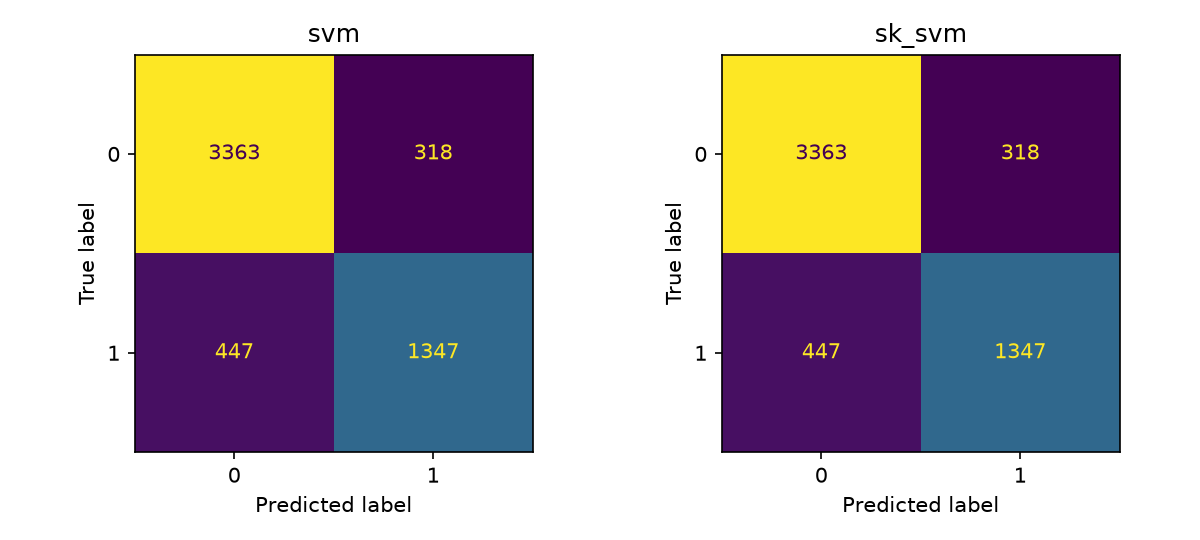
\includegraphics[width=0.85\textwidth]{confusion_svm}
	\caption{\textit{Confusion matrix} SVM \textit{from scratch} (kiri) dan \texttt{SVC} (kanan) pada \texttt{X\_val}}
	\label{fig:cm-svm}
\end{figure}

\begin{table}[H]
	\centering
	\caption{\textit{Classification report} SVM pada \texttt{X\_val} (sama untuk \textit{from scratch} dan \texttt{SVC})}
	\label{tab:report-svm}
	\begin{tabular}{l c c c r}
		\toprule
		\textbf{Kelas} & \textbf{\textit{Precision}} & \textbf{\textit{Recall}} & \textbf{F1} & \textbf{\textit{Support}} \\
		\midrule
		0 (tidak batal) & 0,8827 & 0,9136 & 0,8979 & 3.681 \\
		1 (batal)       & 0,8090 & 0,7508 & 0,7788 & 1.794 \\
		\midrule
		\textit{Accuracy}     & \multicolumn{3}{c}{0,8603} & 5.475 \\
		\textit{Macro avg}    & 0,8458 & 0,8322 & 0,8384 & 5.475 \\
		\bottomrule
	\end{tabular}
\end{table}

\subsection{Analisis}

Dari 1.794 pembatalan pada \texttt{X\_val}, SVM mendeteksi 1.347 pembatalan
(\textit{recall} 75\%) dan melewatkan 447 pembatalan (\textit{false negative}).
Sebanyak 318 pemesanan yang tidak batal salah diprediksi batal (\textit{false
positive}). F1 kelas batal (0,78) lebih rendah daripada F1 kelas tidak batal
(0,90). Kelas batal juga merupakan kelas yang jumlah sampelnya lebih sedikit.

Simpangan baku antar-\textit{fold} kecil (0,006), dan skor \textit{hold-out} dekat
dengan rata-rata \textit{k-fold}. Kinerja SVM tidak bergantung pada satu cara
pembagian data tertentu.

SVM RBF mengungguli Logistic Regression scikit-learn (0,8384 dan 0,7713). Selisih
ini mengindikasikan bahwa batas keputusan antara kedua kelas tidak linear sehingga
model linear dengan fitur yang sama tidak dapat menangkapnya sepenuhnya.

\texttt{GaussianNB} hanya mencapai 0,3773. Model ini mengasumsikan setiap fitur
berdistribusi normal dan saling bebas jika kelasnya diketahui. Banyak fitur pada
data ini berupa kolom \textit{one-hot} atau fitur diskret yang hampir konstan.
Kemungkinan penyebabnya adalah variansi yang sangat kecil pada fitur-fitur
tersebut sehingga \textit{likelihood}-nya mendominasi posterior. Dugaan ini belum
diuji.

\subsection{Seleksi Fitur SVM}

SVM linear ($C=0{,}1$) yang dilatih dengan tiga puluh fitur menghasilkan sepuluh
fitur dengan $|w|$ terbesar. Urutannya dari yang terbesar adalah
\texttt{special\_requests}, \texttt{days\_before\_arrival}, \texttt{date\_rate},
\texttt{lead\_x\_price}, \texttt{booking\_channel\_Online Travel Agent},
\texttt{booking\_channel\_Offline Agent}, \texttt{booking\_channel\_Complimentary},
\texttt{needs\_parking}, \texttt{is\_returning\_guest}, dan \texttt{doy\_cos}.
Dua fitur teratas sama dengan dua fitur yang nilai mutlak korelasinya terhadap
target paling besar pada Bab~1. Dua fitur hasil rekayasa, yaitu \texttt{date\_rate} dan
\texttt{lead\_x\_price}, berada di peringkat ketiga dan keempat.

Untuk melihat apakah seleksi fitur dan reduksi dimensi membantu, SVM RBF ($C=3$,
$\gamma=0{,}1$) dilatih dengan empat variasi masukan (Tabel~\ref{tab:seleksi}).
SVM RBF tidak memiliki bobot $w$ sehingga \texttt{Pipeline(select=k)} tidak dapat
meranking fiturnya sendiri. Karena itu, pada varian top-$k$, peringkat fitur
diambil dari $|w|$ SVM linear ($C=0{,}1$), lalu SVM RBF dilatih dengan $k$ fitur
teratas. Peringkat ini dihitung ulang pada setiap \textit{fold} agar data validasi
tidak ikut menentukan fitur yang dipilih. Varian PCA memakai
\texttt{Pipeline(pca=0.95)}, yang memilih 21 komponen untuk menjelaskan 95\%
variansi. Sebagai pembanding, SVM linear juga dievaluasi dengan tiga puluh fitur
dan dengan \texttt{Pipeline(select=10)}.

\begin{table}[H]
	\centering
	\caption{Pengaruh seleksi fitur dan PCA pada SVM}
	\label{tab:seleksi}
	\begin{tabular}{l l c c c}
		\toprule
		\textbf{Model} & \textbf{Masukan} & \textbf{\textit{Hold-out}} & \textbf{5-\textit{fold} $\mu$} & \textbf{5-\textit{fold} $\sigma$} \\
		\midrule
		SVM RBF    & 30 fitur                   & \textbf{0,8384} & \textbf{0,8328} & 0,0062 \\
		SVM RBF    & PCA (21 komponen)          & 0,8376 & 0,8305 & 0,0062 \\
		SVM RBF    & 20 fitur teratas           & 0,8219 & 0,8214 & 0,0042 \\
		SVM RBF    & 10 fitur teratas           & 0,7964 & 0,8013 & 0,0083 \\
		\midrule
		SVM linear & 30 fitur                   & 0,7705 & 0,7667 & 0,0077 \\
		SVM linear & 10 fitur teratas           & 0,7676 & 0,7651 & 0,0081 \\
		\bottomrule
	\end{tabular}
\end{table}

Seleksi fitur tidak membantu SVM RBF. Dengan dua puluh fitur teratas, rata-rata
5-\textit{fold} turun 0,0114, dan dengan sepuluh fitur teratas turun 0,0315.
Kemungkinan penyebabnya, peringkat dari SVM linear hanya mengukur kontribusi
linear setiap fitur, sedangkan fitur yang bobot linearnya kecil masih dapat
berguna bagi kernel RBF melalui interaksinya dengan fitur lain. Pada SVM
linear, seleksi sepuluh fitur hampir tidak mengubah skor (0,7651 dan 0,7667)
karena peringkatnya berasal dari model yang sama.

PCA dengan 21 komponen menghasilkan skor yang hampir sama dengan tiga puluh fitur
asli. Selisih rata-ratanya (0,0023) lebih kecil daripada simpangan baku
antar-\textit{fold} (0,0062). PCA mengurangi dimensi masukan sepertiga tanpa
penurunan skor yang berarti, tetapi juga tidak menaikkan skor. Karena itu, model
akhir tetap memakai tiga puluh fitur tanpa seleksi dan tanpa PCA.

\section{Hasil Bayesian Network}
\label{sec:hasil-bn}

\subsection{TAN Dibandingkan \textit{Naive Bayes}}

\textit{Naive Bayes} dan TAN memakai diskretisasi, CPT, dan 5 \textit{bin} yang
sama. Satu-satunya perbedaan adalah struktur: TAN menambahkan satu
\textit{parent} fitur per fitur (Subbab~\ref{sec:tan}). Pada Tabel~\ref{tab:perbandingan},
TAN mencapai \textit{macro F1} 5-\textit{fold} 0,7624 ($\sigma=0{,}0066$)
berbanding 0,7119 ($\sigma=0{,}0049$) untuk \textit{Naive Bayes}. Selisih 0,0505
jauh lebih besar daripada simpangan baku antar-\textit{fold}. Pada \textit{hold-out},
selisihnya 0,0634 (0,7617 berbanding 0,6983). Besarnya berbeda dari 5-\textit{fold},
tetapi arahnya sama pada kedua cara evaluasi.

Diskretisasi juga memperbaiki \textit{Naive Bayes} secara besar dibandingkan
\texttt{GaussianNB} (0,7119 berbanding 0,3804) dengan asumsi kebebasan yang sama.
Hasil ini sejalan dengan dugaan pada bab sebelumnya bahwa distribusi normal tidak
cocok untuk fitur \textit{one-hot} dan fitur diskret pada data ini. Dugaan
tersebut belum diuji secara langsung.

\begin{table}[H]
	\centering
	\caption{\textit{Classification report} \textit{Naive Bayes}, TAN, dan KDB ($k=10$) pada \texttt{X\_val}}
	\label{tab:report-bn}
	\begin{tabular}{l l c c c}
		\toprule
		\textbf{Model} & \textbf{Kelas} & \textbf{\textit{Precision}} & \textbf{\textit{Recall}} & \textbf{F1} \\
		\midrule
		\textit{Naive Bayes} & 0 (tidak batal) & 0,8246 & 0,7446 & 0,7826 \\
		                     & 1 (batal)       & 0,5630 & 0,6750 & 0,6139 \\
		\midrule
		TAN                  & 0 (tidak batal) & 0,8374 & 0,8587 & 0,8479 \\
		                     & 1 (batal)       & 0,6941 & 0,6577 & 0,6754 \\
		\midrule
		KDB ($k=10$)         & 0 (tidak batal) & 0,8550 & 0,9242 & 0,8883 \\
		                     & 1 (batal)       & 0,8135 & 0,6784 & 0,7398 \\
		\bottomrule
	\end{tabular}
\end{table}

\textit{Naive Bayes} memprediksi 39,3\% baris \texttt{X\_val} sebagai batal,
padahal proporsi pembatalan sebenarnya 32,8\%. Kelebihan prediksi batal ini
terlihat pada \textit{precision} kelas batal yang rendah (0,5630) dan 940
\textit{false positive}. TAN memprediksi 31,1\% baris sebagai batal, hampir sama
dengan proporsi sebenarnya, dengan \textit{false positive} turun menjadi 520.
Penyebab yang mungkin adalah informasi ganda dari fitur yang saling berkaitan
pada \textit{Naive Bayes}. Penyebab ini sejalan dengan struktur TAN pada
Subbab berikutnya, tetapi belum diuji dengan menghapus fitur yang berkaitan.

\subsection{Struktur yang Dipelajari TAN}

Dari 666 pasangan fitur yang mungkin, TAN memilih 36 edge. Edge dengan
\textit{conditional mutual information} terbesar adalah pasangan fitur yang
diturunkan dari fitur yang sama: \texttt{arrival\_month} $\to$ \texttt{month\_cos}
(1,150), \texttt{month\_sin} $\to$ \texttt{doy\_sin} (1,113),
\texttt{arrival\_month} $\to$ \texttt{month\_sin} (1,093), dan
\texttt{month\_cos} $\to$ \texttt{doy\_cos} (0,867). Pasangan berikutnya juga
bersifat turunan: \texttt{num\_adults} $\to$ \texttt{total\_guests} (0,609),
\texttt{weekday\_nights} $\to$ \texttt{total\_nights} (0,494), dan
\texttt{lead\_x\_price} $\to$ \texttt{days\_before\_arrival} (0,333). Ada pula
pasangan dua kolom \textit{one-hot} dari satu atribut, yaitu
\texttt{booking\_channel\_Online Travel Agent} $\to$
\texttt{booking\_channel\_Offline Agent} (0,432): jika satu kolom bernilai 1,
kolom lain pasti 0. Ini adalah pasangan yang menyebabkan \textit{Naive Bayes}
menghitung informasi yang sama berulang kali. Nilai terkecil di antara edge
terpilih kurang dari 0,001, yaitu hubungan yang hampir tidak ada
(Gambar~\ref{fig:graf-bn}).

Harga dari struktur ini adalah ukuran tabel. Jumlah sel CPT (seluruh nilai
probabilitas yang disimpan) naik dari 240 pada \textit{Naive Bayes} menjadi 918
pada TAN. CPT terbesar berukuran
$2\times5\times5=50$ sel (misalnya pada \texttt{days\_before\_arrival}).
Tabel yang lebih besar membutuhkan data lebih banyak, tetapi dengan 21.898 baris
latih ini belum menimbulkan masalah yang terlihat.

\subsection{KDB: Lebih dari Satu \textit{Parent}}
\label{sec:hasil-kdb}

KDB (Subbab~\ref{sec:kdb}) dievaluasi dengan diskretisasi dan 5 \textit{bin}
yang sama, sehingga satu-satunya perbedaan dengan TAN adalah jumlah
\textit{parent} fitur. Tabel~\ref{tab:kdb} menunjukkan pengaruh $k$.

\begin{table}[H]
	\centering
	\caption{Pengaruh $k$ pada KDB (\texttt{n\_bins}=5, \textit{macro F1})}
	\label{tab:kdb}
	\begin{tabular}{c c c c r}
		\toprule
		$k$ & \textbf{\textit{Hold-out}} & \textbf{5-\textit{fold} $\mu$} & \textbf{5-\textit{fold} $\sigma$} & \textbf{Sel CPT padat} \\
		\midrule
		0 (\textit{Naive Bayes}) & 0,6983 & 0,7119 & 0,0049 & 240 \\
		1 & 0,7630 & 0,7695 & 0,0041 & 968 \\
		2 & 0,7718 & 0,7744 & 0,0080 & 4.312 \\
		3 & 0,7826 & 0,7836 & 0,0045 & 18.476 \\
		4 & 0,7827 & 0,7925 & 0,0051 & 60.840 \\
		5 & 0,7893 & 0,7956 & 0,0019 & 221.990 \\
		6 & 0,8023 & 0,8009 & 0,0078 & 911.060 \\
		8 & 0,8069 & 0,8032 & 0,0022 & $1{,}3\times10^{7}$ \\
		\textbf{10} & \textbf{0,8140} & \textbf{0,8117} & 0,0072 & $1{,}7\times10^{8}$ \\
		12 & 0,8125 & 0,8101 & 0,0051 & $1{,}7\times10^{9}$ \\
		16 & 0,8041 & 0,8006 & 0,0043 & $2{,}7\times10^{11}$ \\
		29 & 0,7930 & 0,7937 & 0,0056 & $3{,}1\times10^{16}$ \\
		\bottomrule
	\end{tabular}
\end{table}

Skor naik seiring $k$ sampai sekitar $k=10$, lalu turun. Dari TAN (0,7624) ke KDB
$k=10$ (0,8117), \textit{macro F1} 5-\textit{fold} naik 0,0493, tujuh kali
simpangan bakunya. KDB $k=1$ (0,7695) sedikit di atas TAN walaupun keduanya
memberi satu \textit{parent} per fitur. Bedanya, KDB memilih \textit{parent}
berdasarkan urutan $I(X_i;C)$, sedangkan TAN memilih pohon dengan total bobot
terbesar.

Penurunan setelah $k=10$ sejalan dengan jumlah data. Dengan 21.898 baris latih,
makin banyak \textit{parent}, makin sedikit baris yang jatuh pada setiap
kombinasi nilai \textit{parent}. Sel CPT padat pada $k=10$ sudah
$1{,}7\times10^{8}$, sedangkan hitungan yang benar-benar tersimpan sebagai CPT
\textit{sparse} hanya sekitar 430 ribu. Sebagian besar peluang akhirnya hanya
berasal dari \textit{smoothing}. Nilai di sekitarnya hampir setara: $k=9$
mendapat 0,8059, $k=11$ mendapat 0,8125, dan $k=12$ mendapat 0,8101. Selisih
terbesarnya 0,0066, sebanding dengan simpangan baku, sehingga rentang $k=9$
sampai 12 tidak dapat dibedakan secara meyakinkan.

Nilai $k=10$ dipilih sebagai model akhir karena berada di rentang tersebut dengan
CPT lebih kecil daripada $k=11$ dan $k=12$. Pada $k=10$, \texttt{alpha} 0,5 dan 2
memberi 0,8085 dan 0,8120, sehingga \texttt{alpha}=1 dipertahankan. Nilai
\texttt{n\_bins} 4 dan 6 memberi 0,8119 dan 0,8070. Empat \textit{bin} setara
dengan lima, sehingga 5 \textit{bin} dipertahankan agar sama dengan
\textit{Naive Bayes} dan TAN.

Pada \texttt{X\_val}, KDB $k=10$ mencapai akurasi 0,8437 dan memprediksi 27,3\%
baris sebagai batal. \textit{Precision} kelas batal naik menjadi 0,8135
(TAN 0,6941) dan \textit{recall}-nya juga naik menjadi 0,6784 (TAN 0,6577).
\textit{False positive} turun dari 520 pada TAN menjadi 279.

\todo{Isi skor Kaggle KDB $k=10$ dari \texttt{output/bn\_kdb10.csv} setelah
berkas itu diunggah, lalu bandingkan dengan \textit{macro F1} \textit{hold-out}
(0,8140).}

\subsection{Pengaruh \texttt{n\_bins}}
\label{sec:tuning-bn}

Jumlah \textit{bin} dipilih dengan \textit{grid search} 5-\textit{fold}
(Tabel~\ref{tab:tuning-bn}).

\begin{table}[H]
	\centering
	\caption{Hasil \textit{tuning} \texttt{n\_bins} pada Bayesian Network}
	\label{tab:tuning-bn}
	\begin{tabular}{c c c c c}
		\toprule
		& \multicolumn{2}{c}{\textbf{\textit{Naive Bayes}}} & \multicolumn{2}{c}{\textbf{TAN}} \\
		\cmidrule(lr){2-3}\cmidrule(lr){4-5}
		\textbf{\texttt{n\_bins}} & \textbf{5-\textit{fold} $\mu$} & \textbf{5-\textit{fold} $\sigma$} & \textbf{5-\textit{fold} $\mu$} & \textbf{5-\textit{fold} $\sigma$} \\
		\midrule
		3  & \textbf{0,7148} & 0,0070 & 0,7460 & 0,0056 \\
		5  & 0,7119 & 0,0049 & \textbf{0,7624} & 0,0066 \\
		10 & 0,7116 & 0,0042 & 0,7570 & 0,0056 \\
		\bottomrule
	\end{tabular}
\end{table}

Pada \textit{Naive Bayes}, ketiga nilai \texttt{n\_bins} praktis setara karena
selisih terbesar (0,0032) lebih kecil daripada simpangan baku (0,004--0,007).
Pada TAN, \texttt{n\_bins}=5 terbaik, sedangkan 3 \textit{bin} turun 0,0164 dan 10
\textit{bin} turun 0,0054. Penurunan pada 10 \textit{bin} masih sebanding dengan
simpangan baku, sehingga hanya 3 \textit{bin} yang jelas lebih buruk.
Kemungkinan penyebabnya, 3 \textit{bin} terlalu kasar untuk menangkap hubungan
antarfitur. Dugaan ini belum diuji.

\subsection{Klasifikasi Sensitif-Biaya}

Aturan keputusan dengan $C_{FP}=2$ dan $C_{FN}=1$ (Subbab~\ref{sec:biaya-bn}) dievaluasi pada
\texttt{X\_val} dengan biaya total $2\cdot FP+FN$ (Tabel~\ref{tab:biaya-bn}).

\begin{table}[H]
	\centering
	\caption{Pengaruh aturan keputusan sensitif-biaya pada \texttt{X\_val} (Batal = persentase baris yang diprediksi batal)}
	\label{tab:biaya-bn}
	\small
	\begin{tabular}{l r r r c c}
		\toprule
		\textbf{Model} & \textbf{FP} & \textbf{FN} & \textbf{Biaya $2\,FP+FN$} & \textbf{\textit{Macro F1}} & \textbf{Batal (\%)} \\
		\midrule
		\textit{Naive Bayes}              & 940 & 583 & 2.463 & 0,6983 & 39,3 \\
		\textit{Naive Bayes} + biaya      & 704 & 689 & 2.097 & 0,7119 & 33,0 \\
		TAN                               & 520 & 614 & 1.654 & 0,7617 & 31,1 \\
		TAN + biaya                       & 285 & 845 & 1.415 & 0,7421 & 22,5 \\
		KDB ($k=10$)                      & 279 & 577 & 1.135 & 0,8140 & 27,3 \\
		KDB ($k=10$) + biaya              & 222 & 626 & 1.070 & 0,8122 & 25,4 \\
		\bottomrule
	\end{tabular}
\end{table}

Aturan sensitif-biaya menurunkan biaya total pada ketiga model: dari 2.463 ke 2.097
(turun 14,9\%) pada \textit{Naive Bayes}, dari 1.654 ke 1.415 (turun 14,5\%)
pada TAN, dan dari 1.135 ke 1.070 (turun 5,7\%) pada KDB. Penurunan pada KDB
paling kecil karena KDB sudah lebih jarang memprediksi batal (279
\textit{false positive}). \textit{False positive} turun dan \textit{false negative}
naik, sesuai dengan harga yang diasumsikan. \textit{Macro F1} tidak otomatis ikut
naik: pada TAN justru turun (0,7617 menjadi 0,7421) karena \textit{macro F1}
menganggap semua kesalahan sama berat, sedangkan yang dioptimalkan adalah biaya.
Pada \textit{Naive Bayes} \textit{macro F1} naik (0,6983 menjadi 0,7119) karena
model ini semula terlalu sering memprediksi batal. Pemilihan antara
\textit{macro F1} dan biaya bergantung pada metrik yang dianggap utama. Metrik
penilaian tugas ini adalah \textit{macro F1}, sehingga aturan sensitif-biaya
dilaporkan sebagai bonus dan tidak dipakai pada perbandingan utama
(Tabel~\ref{tab:perbandingan}).

\section{\textit{Hyperparameter Tuning}}

\textit{Tuning} dijalankan dengan fungsi \texttt{tune}, yaitu \textit{grid search}
yang menilai setiap kombinasi parameter dengan rata-rata \textit{macro F1}
5-\textit{fold} pada \texttt{X\_train}. Untuk SVM, \textit{grid} pada
\textit{notebook} memvariasikan $C\in\{1,3,5\}$ dengan kernel RBF dan
$\gamma=0{,}1$ tetap (Tabel~\ref{tab:tuning-svm}). Kelima belas pelatihan
(tiga kombinasi $\times$ lima \textit{fold}) selesai dalam 172 detik.

\begin{table}[H]
	\centering
	\caption{Hasil \textit{tuning} SVM RBF ($\gamma=0{,}1$)}
	\label{tab:tuning-svm}
	\begin{tabular}{c c c}
		\toprule
		$C$ & \textbf{5-\textit{fold} $\mu$} & \textbf{5-\textit{fold} $\sigma$} \\
		\midrule
		1 & 0,8288 & 0,0034 \\
		3 & \textbf{0,8328} & 0,0062 \\
		5 & 0,8322 & 0,0064 \\
		\bottomrule
	\end{tabular}
\end{table}

Nilai $C=3$ memberikan rata-rata tertinggi (0,8328) dan dipilih sebagai
konfigurasi akhir. Menaikkan $C$ dari 1 ke 3 menambah 0,0040, sedangkan menaikkan
$C$ dari 3 ke 5 justru menurunkan skor sebesar 0,0006. Selisih antara $C=3$ dan
$C=5$ jauh lebih kecil daripada simpangan baku antar-\textit{fold} (sekitar
0,006) sehingga keduanya praktis setara. Semakin besar $C$, semakin besar pula
hukuman untuk sampel yang melanggar margin. Pada rentang ini, kenaikan $C$ di atas
3 tidak lagi memperbaiki skor validasi.

Model akhir ($C=3$) yang dilatih pada \texttt{X\_train} konvergen setelah 30.419
iterasi SMO dan memiliki 9.039 \textit{support vector} (41\% dari 21.857 baris).
Sebanyak 5.131 di antaranya memiliki $\alpha=C$, yaitu sampel yang berada di
dalam margin atau salah diklasifikasikan pada data latih. Jumlah ini mengindikasikan
bahwa kedua kelas banyak beririsan pada ruang fitur.

\todo{Tambahkan hasil \textit{tuning} KNN ($k\in\{5,15,31\}$), Logistic Regression
($\texttt{lr}\in\{0{,}01;0{,}1\}$), dan DTL ($\texttt{max\_depth}\in\{5,8,\text{None}\}$)
serta tabel \texttt{ranking} semua model. \textit{Tuning} Bayesian Network ada pada
Subbab~\ref{sec:tuning-bn}.}

\section{Analisis Kesalahan}

SVM hasil \textit{tuning} salah memprediksi 765 dari 5.475 baris \texttt{X\_val}
(14,0\%), terdiri atas 447 \textit{false negative} dan 318 \textit{false
positive} (Gambar~\ref{fig:cm-svm}). Jumlah \textit{false negative} yang lebih
besar sesuai dengan proporsi prediksi batal: model memprediksi 30,4\% baris
\texttt{X\_val} sebagai batal, sedangkan proporsi pembatalan sebenarnya 32,8\%.

Untuk mencari pola kesalahan, baris \texttt{X\_val} dikelompokkan menjadi
\textit{true positive} (TP), \textit{true negative} (TN), \textit{false positive}
(FP), dan \textit{false negative} (FN), lalu nilai fitur aslinya dibandingkan.
Median \textit{lead time} kelompok TP adalah 161 hari dan kelompok TN 37 hari.
Kesalahan berada di antara keduanya: median FN 62 hari dan median FP 80 hari.
Pola yang sama terlihat pada permintaan khusus. Proporsi pemesanan tanpa
permintaan khusus adalah 68,6\% pada TP dan 37,8\% pada TN, sedangkan pada FP
61,3\% dan pada FN 42,3\%. Dengan kata lain, pembatalan yang terlewat (FN) memiliki
ciri yang mirip dengan pemesanan yang tidak batal, dan pemesanan yang salah
diprediksi batal (FP) memiliki ciri yang mirip dengan pembatalan.

\begin{table}[H]
	\centering
	\caption{Tingkat kesalahan SVM pada \texttt{X\_val} berdasarkan \textit{lead time}}
	\label{tab:error-lead}
	\begin{tabular}{l r c c r r}
		\toprule
		\textbf{\textit{Lead time} (hari)} & \textbf{Baris} & \textbf{Rasio batal} & \textbf{Tingkat kesalahan} & \textbf{FN} & \textbf{FP} \\
		\midrule
		0-7     & 802   & 0,086 & 0,072 & 42  & 16 \\
		8-30    & 965   & 0,181 & 0,123 & 71  & 48 \\
		31-90   & 1.562 & 0,256 & 0,159 & 149 & 99 \\
		91-180  & 1.133 & 0,457 & 0,211 & 122 & 117 \\
		$>180$   & 767   & 0,722 & 0,065 & 24  & 26 \\
		\bottomrule
	\end{tabular}
\end{table}

Tabel~\ref{tab:error-lead} menunjukkan bahwa tingkat kesalahan tertinggi
(21,1\%) terjadi pada \textit{lead time} 91-180 hari, yaitu rentang dengan rasio
pembatalan paling dekat dengan 50\%. Pada \textit{lead time} sangat pendek
($\le 7$ hari) dan sangat panjang ($>180$ hari), sebagian besar pemesanan berada
di satu kelas sehingga tingkat kesalahannya di bawah 8\%. Sebanyak 246 baris
dengan \textit{lead time} kosong pada data mentah tidak masuk ke tabel ini.

Tingkat kesalahan juga berbeda antarkanal pemesanan. Tingkat kesalahan pada Online
Travel Agent adalah 17,9\% (3.519 baris), sedangkan pada Offline Agent 6,9\%
(1.573 baris) dan pada Corporate 8,1\% (309 baris). Rasio pembatalan Online Travel
Agent (36,2\%) dan Offline Agent (30,8\%) tidak jauh berbeda, tetapi pembatalan
pada Online Travel Agent lebih sulit dipisahkan oleh fitur yang tersedia. Fitur
tambahan yang membedakan pemesanan pada kanal ini dapat menjadi arah perbaikan.

\todo{Tambahkan \textit{confusion matrix} model lain setelah \textit{tuning}.}

\section{Prediksi Data Uji}

Model akhir, yaitu SVM RBF dengan $C=3$ dan $\gamma=0{,}1$, dilatih ulang dengan
gabungan \texttt{X\_train} dan \texttt{X\_val} (27.332 baris). Pelatihan ini
konvergen setelah 37.842 iterasi SMO dengan 10.927 \textit{support vector}.
Prediksi untuk 6.844 baris \texttt{X\_test} disimpan di
\texttt{output/svm\_20261121-120000.csv}, dan modelnya disimpan di berkas
\texttt{.pkl} dengan nama yang sama. Model memprediksi 29,8\% baris data uji
sebagai batal, mendekati proporsi prediksi batal pada \texttt{X\_val} (30,4\%).

Prediksi pada berkas ini identik dengan prediksi pada submisi Kaggle sebelumnya
(\texttt{svm\_20261120-214807.csv}) untuk seluruh 6.844 baris. Submisi tersebut
memperoleh skor 0,84979 pada Kaggle. Skor tersebut lebih
tinggi daripada \textit{macro F1} \textit{hold-out} (0,8384) dan rata-rata
5-\textit{fold} (0,8328). Salah satu kemungkinan penyebabnya adalah jumlah data
latih model akhir yang 25\% lebih banyak, tetapi selisih ini juga dapat berasal
dari perbedaan sampel data uji.


	\chapter{Kesimpulan dan Saran}
	\section{Kesimpulan}

\begin{enumerate}
	\item SVM \textit{soft margin} telah diimplementasikan \textit{from scratch}
	dengan SMO dan \textit{second-order working set selection}. Implementasi ini
	mendukung kernel linear, polinomial, RBF/Gaussian, dan sigmoid. Dengan
	\textit{hyperparameter} yang sama, \textit{macro F1}-nya identik dengan
	\texttt{sklearn.svm.SVC}, yaitu 0,8384 pada \textit{hold-out} dan 0,8328 pada
	5-\textit{fold cross validation}.
	\item Semua tahap \textit{preprocessing} di-\textit{fit} hanya pada data latih.
	\textit{Target encoding} tanggal kedatangan dihitung secara
	\textit{out-of-fold} agar label setiap baris tidak bocor ke fiturnya sendiri.
\end{enumerate}

\todo{Tambahkan kesimpulan untuk KNN, Logistic Regression, DTL, dan Bayesian
Network, serta model terbaik secara keseluruhan setelah \textit{tuning}.}

\section{Saran}

\begin{enumerate}
	\item \textit{Recall} kelas batal (75\%) lebih rendah daripada
	\textit{precision}-nya (81\%). Ambang \texttt{decision\_function} dapat digeser
	dari 0, atau nilai $C$ dapat dibedakan per kelas. Kedua cara ini perlu diuji
	untuk melihat apakah \textit{macro F1} naik.
\end{enumerate}

\todo{Tambahkan saran dari hasil algoritma lain.}


	\chapter{Pembagian Tugas}
	\begin{table}[H]
	\centering
	\caption{Pembagian tugas anggota kelompok}
	\label{tab:pembagian}
	\begin{tabular}{l l p{6cm}}
		\toprule
		\textbf{Nama} & \textbf{NIM} & \textbf{Tugas} \\
		\midrule
		Jason Edward Salim & 13524034 & Support Vector Machine \\
		Stefani Angeline Oroh & 13524064 & Logistic Regression (model \textit{from scratch}, rekayasa fitur c010, dan perbandingan \textit{solver}) \\
		Bryan Pratama Putra Hendra & 13524067 & K-Nearest Neighbors dan optimasinya, merapikan \textit{notebook} \\
		Angelina Andra Alanna & 13524079 & Bayesian Network (\textit{Naive Bayes}, TAN, KDB, graf, sensitif-biaya) \\
		Michael James Liman & 13524106 & Decision Tree Learning dan optimasinya, visualisasi pohon (bonus), peningkatan skor Kaggle hingga peringkat tiga besar \\
		\bottomrule
	\end{tabular}
\end{table}


	\bibliography{dafpus}

	\appendix
	\chapter{Lampiran}
	\section{Tautan \textit{Repository}}

\url{https://github.com/jsndwrd/IF3170_G08_Teazzi}

\section{Pernyataan Penggunaan AI Generatif}

Kelompok menggunakan asisten AI generatif selama pengerjaan tugas ini. Seluruh
keluaran AI telah diperiksa, dijalankan, dan dipahami oleh anggota kelompok. Surat
pernyataan pada subbab berikutnya mengikuti format Panduan Penggunaan
\textit{Generative AI} ITB~\cite{itb2024panduanai}.

\begin{table}[H]
	\centering
	\caption{Penggunaan AI generatif}
	\label{tab:genai}
	\begin{tabular}{p{2.5cm} p{10.7cm}}
		\toprule
		\textbf{Alat} & \textbf{Penggunaan} \\
		\midrule
		Claude & Membantu menyusun kerangka laporan. \\
		\bottomrule
	\end{tabular}
\end{table}

% ---------- Surat pernyataan (format Panduan AI ITB) ----------
% Tanda tangan: simpan gambar di docs/public/ttd/<NIM>.png (latar transparan atau putih).
\newcommand{\ttdanggota}[2]{%
	\begin{minipage}[t]{6.5cm}
		\centering
		\IfFileExists{public/ttd/#2.png}{%
			\includegraphics[height=2cm,width=5.5cm,keepaspectratio]{ttd/#2}%
		}{%
			\rule{0pt}{2cm}%
		}\\[2pt]
		\rule{5.5cm}{0.4pt}\\[2pt]
		#1\\
		#2
	\end{minipage}%
}

\clearpage
\section{Surat Pernyataan Penggunaan AI}
\noindent Dengan ini, kami:

\noindent
\begin{tabular}{@{}l l@{}}
	Nama/NIM            & : 1. Jason Edward Salim/13524034 \\
	                    & \phantom{:} 2. Stefani Angeline Oroh/13524064 \\
	                    & \phantom{:} 3. Bryan Pratama Putra Hendra/13524067 \\
	                    & \phantom{:} 4. Angelina Andra Alanna/13524079 \\
	                    & \phantom{:} 5. Michael James Liman/13524106 \\
	Fakultas/Sekolah    & : Sekolah Teknik Elektro dan Informatika \\
	Kode Mata Kuliah    & : IF3170 \\
	Nama Mata Kuliah    & : Inteligensi Artifisial \\
	Judul Tugas         & : Tugas Besar 2 IF3170 Inteligensi Artifisial 2026/2027 \\
\end{tabular}

\medskip
\noindent menyatakan bahwa kami menggunakan AI dalam pengerjaan maupun penyusunan
luaran tugas pada mata kuliah yang tertulis di atas.

\medskip
\noindent Jika ya, alat AI/kecerdasan buatan yang digunakan adalah:

\begin{center}
\small
\renewcommand{\arraystretch}{1.25}
\begin{tabular}{|>{\raggedright\arraybackslash}p{5.3cm}|>{\centering\arraybackslash}p{2.4cm}|>{\raggedright\arraybackslash}p{5.4cm}|}
	\hline
	\multicolumn{1}{|c|}{\textbf{Lingkup Pekerjaan}} & \textbf{Digunakan?} & \multicolumn{1}{c|}{\textbf{Tingkat Penggunaan}} \\
	\hline
	Pemeriksaan Ejaan: menggunakan \textit{tools} seperti Grammarly, Paperpal,
	DeepL, Quillbot, Grammarbot, LanguageTool, ProWritingAid, ChatGPT, Google
	Gemini, atau sejenisnya.
	& Tidak
	& \\
	\hline
	Pembuatan Teks: menggunakan \textit{tools} seperti ChatGPT, Gemini, Paperpal,
	Copilot, GrammarlyGO, WordAI, WriteSonic, Jasper, Jenni AI, atau sejenisnya.
	& Ya
	& Membantu menyusun kerangka laporan. \\
	\hline
	Bantuan Diskusi dalam Penyusunan Konten: menggunakan \textit{tools} seperti
	ChatGPT, Gemini, Copilot, Perplexity, Jenni AI, Zoom-Companion, atau
	sejenisnya.
	& Ya
	& Mempelajari cara kerja algoritma supervised learning secara mendalam sebelum dikembangkan menjadi barisan kode. \\
	\hline
	Pembuatan Gambar, Video, dan/atau Grafik: menggunakan \textit{tools} seperti
	Craiyon, DALL-E, Midjourney, Stable Diffusion, Microsoft Designer, Gemini,
	Canva AI, atau sejenisnya.
	& Tidak
	& \\
	\hline
	Lainnya, jelaskan:
	& Tidak
	& - \\
	\hline
\end{tabular}
\end{center}

\noindent Kami juga menyatakan bahwa setiap penggunaan AI/kecerdasan buatan yang
dilakukan pada mata kuliah tersebut telah dinyatakan di dalam surat ini.

\bigskip
\begin{flushright}
	Bandung, 23 November 2026
\end{flushright}

\bigskip
\noindent
\begin{center}
	\ttdanggota{Jason Edward Salim}{13524034}\hspace{1cm}%
	\ttdanggota{Stefani Angeline Oroh}{13524064}

	\vspace{0.8cm}
	\ttdanggota{Bryan Pratama Putra Hendra}{13524067}\hspace{1cm}%
	\ttdanggota{Angelina Andra Alanna}{13524079}

	\vspace{0.8cm}
	\ttdanggota{Michael James Liman}{13524106}
\end{center}


\end{document}
